\documentclass[10pt, border=5mm]{standalone}

% LuaLaTeX fonts
\usepackage{fontspec}
\setmainfont{Stix Two Text}
\usepackage{unicode-math}
\setmathfont{Stix Two Math}

\usepackage{xcolor}
\usepackage{url}

% TikZ
\usepackage{tikz}
\usetikzlibrary{calc,positioning,fit}

% small helpers
\newcommand{\I}{\vphantom{lp}}

\begin{document}

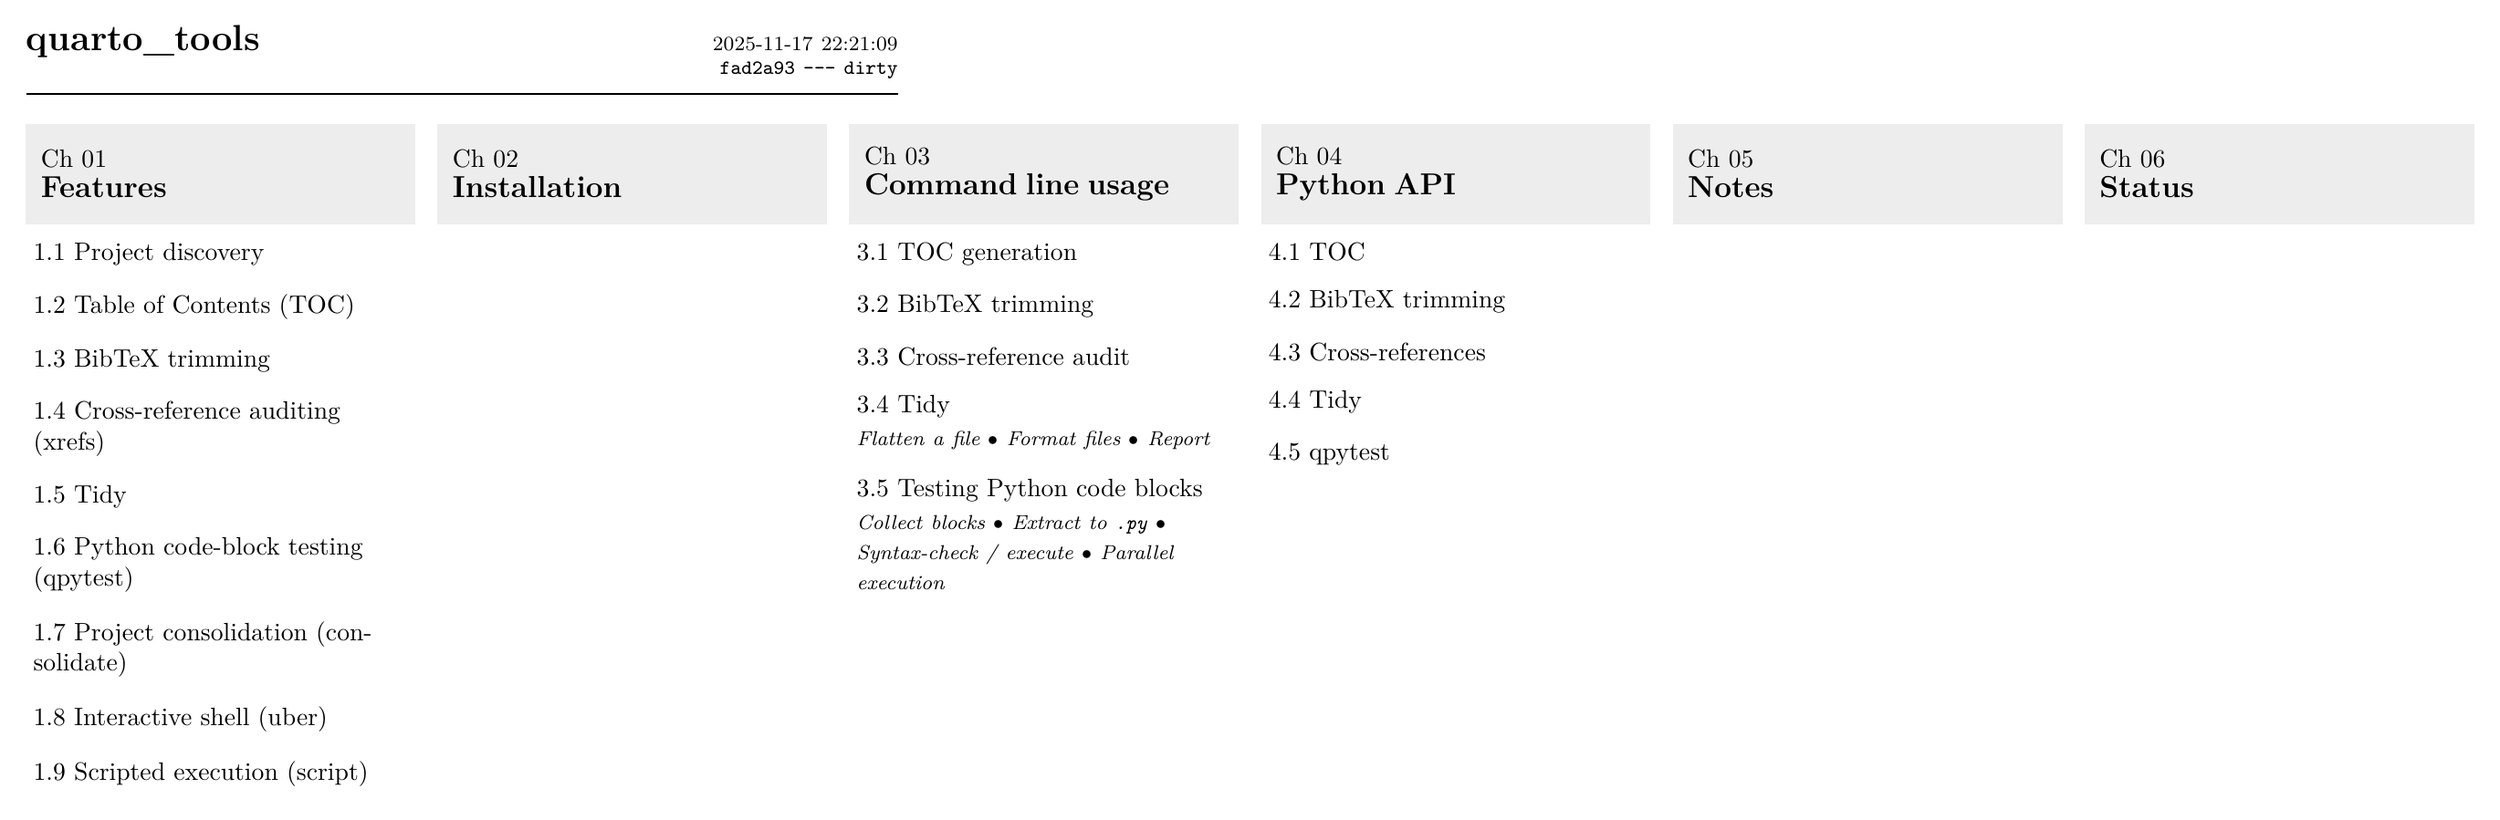
\begin{tikzpicture}[node distance=2mm]
  % requires: \usetikzlibrary{calc,positioning,fit}
  \tikzset{
    tocChapterBox/.style={draw=none, fill=black!7, inner sep=6pt, outer sep=0pt, align=left, text width=5cm, minimum height=1.40cm},
    tocSectionBox/.style={draw=none, inner sep=3pt, outer sep=0pt, text ragged, text width=5cm},
    tocGroupBox/.style={draw=none, inner sep=0pt},
    tocRowBox/.style={draw=none, inner sep=0pt}
  }

% --- Title Bar Node ---
  % Top-left anchored title; spans the full \textwidth
  \node[anchor=north west, inner sep=0pt, text width=\textwidth] (titlebar) at (0,0) {
    \hbox to\textwidth{%
         \vtop{\hsize=.68\textwidth
              \Large\bfseries quarto\_tools\par
         }%
         \hfill
         \vtop{\hsize=.32\textwidth
              \raggedleft\footnotesize 2025-11-17 22:21:09 \\
              \ttfamily fad2a93 --- dirty\par
         }%
    }%
    \vspace{2mm}\hrule\vspace{4mm}\par
  };

  % Row origins: first row line sits just below the title bar
  \coordinate (rowOrigin0) at ($ (titlebar.south west) + (0,-4mm-1.40cm) $);

  \node[tocChapterBox, anchor=south west] (c1-chap) at (rowOrigin0) {Ch 01\\ \large\bfseries Features};

  \node[tocSectionBox, anchor=north west] (c1-sec-1-col0) at ($(c1-chap.south west)+(0,-1.5mm)$) {1.1  Project discovery}; % first in column 0
  \node[tocSectionBox] (c1-sec-2-col0) [below=of c1-sec-1-col0] {1.2  Table of Contents (TOC)};
  \node[tocSectionBox] (c1-sec-3-col0) [below=of c1-sec-2-col0] {1.3  BibTeX trimming};
  \node[tocSectionBox] (c1-sec-4-col0) [below=of c1-sec-3-col0] {1.4  Cross-reference auditing (xrefs)};
  \node[tocSectionBox] (c1-sec-5-col0) [below=of c1-sec-4-col0] {1.5  Tidy};
  \node[tocSectionBox] (c1-sec-6-col0) [below=of c1-sec-5-col0] {1.6  Python code-block testing (qpytest)};
  \node[tocSectionBox] (c1-sec-7-col0) [below=of c1-sec-6-col0] {1.7  Project consolidation (consolidate)};
  \node[tocSectionBox] (c1-sec-8-col0) [below=of c1-sec-7-col0] {1.8  Interactive shell (uber)};
  \node[tocSectionBox] (c1-sec-9-col0) [below=of c1-sec-8-col0] {1.9  Scripted execution (script)};

  \node[tocGroupBox, fit={ (c1-chap) (c1-sec-1-col0) (c1-sec-2-col0) (c1-sec-3-col0) (c1-sec-4-col0) (c1-sec-5-col0) (c1-sec-6-col0) (c1-sec-7-col0) (c1-sec-8-col0) (c1-sec-9-col0) }] (c1-group) {};

  \node[tocChapterBox, anchor=south west] (c2-chap) at ($(c1-group.east|-rowOrigin0)+(3mm,0)$) {Ch 02\\ \large\bfseries Installation};

  \node[tocGroupBox, fit={ (c2-chap) }] (c2-group) {};

  \node[tocChapterBox, anchor=south west] (c3-chap) at ($(c2-group.east|-rowOrigin0)+(3mm,0)$) {Ch 03\\ \large\bfseries Command line usage};

  \node[tocSectionBox, anchor=north west] (c3-sec-1-col0) at ($(c3-chap.south west)+(0,-1.5mm)$) {3.1  TOC generation}; % first in column 0
  \node[tocSectionBox] (c3-sec-2-col0) [below=of c3-sec-1-col0] {3.2  BibTeX trimming};
  \node[tocSectionBox] (c3-sec-3-col0) [below=of c3-sec-2-col0] {3.3  Cross-reference audit};
  \node[tocSectionBox] (c3-sec-4-col0) [below=of c3-sec-3-col0] {3.4  Tidy\\[1pt]{\fontsize{8}{6.0}\selectfont\rmfamily\itshape Flatten a file $\bullet$ Format files $\bullet$ Report}};
  \node[tocSectionBox] (c3-sec-5-col0) [below=of c3-sec-4-col0] {3.5  Testing Python code blocks\\[1pt]{\fontsize{8}{6.0}\selectfont\rmfamily\itshape Collect blocks $\bullet$ Extract to \texttt{.py} $\bullet$ Syntax-check / execute $\bullet$ Parallel execution}};

  \node[tocGroupBox, fit={ (c3-chap) (c3-sec-1-col0) (c3-sec-2-col0) (c3-sec-3-col0) (c3-sec-4-col0) (c3-sec-5-col0) }] (c3-group) {};

  \node[tocChapterBox, anchor=south west] (c4-chap) at ($(c3-group.east|-rowOrigin0)+(3mm,0)$) {Ch 04\\ \large\bfseries Python API};

  \node[tocSectionBox, anchor=north west] (c4-sec-1-col0) at ($(c4-chap.south west)+(0,-1.5mm)$) {4.1  TOC}; % first in column 0
  \node[tocSectionBox] (c4-sec-2-col0) [below=of c4-sec-1-col0] {4.2  BibTeX trimming};
  \node[tocSectionBox] (c4-sec-3-col0) [below=of c4-sec-2-col0] {4.3  Cross-references};
  \node[tocSectionBox] (c4-sec-4-col0) [below=of c4-sec-3-col0] {4.4  Tidy};
  \node[tocSectionBox] (c4-sec-5-col0) [below=of c4-sec-4-col0] {4.5  qpytest};

  \node[tocGroupBox, fit={ (c4-chap) (c4-sec-1-col0) (c4-sec-2-col0) (c4-sec-3-col0) (c4-sec-4-col0) (c4-sec-5-col0) }] (c4-group) {};

  \node[tocChapterBox, anchor=south west] (c5-chap) at ($(c4-group.east|-rowOrigin0)+(3mm,0)$) {Ch 05\\ \large\bfseries Notes};

  \node[tocGroupBox, fit={ (c5-chap) }] (c5-group) {};

  \node[tocChapterBox, anchor=south west] (c6-chap) at ($(c5-group.east|-rowOrigin0)+(3mm,0)$) {Ch 06\\ \large\bfseries Status};

  \node[tocGroupBox, fit={ (c6-chap) }] (c6-group) {};

  % ---- close row 0 ----
  \node[tocRowBox, fit={ (c1-group) (c2-group) (c3-group) (c4-group) (c5-group) (c6-group) }] (rowFit0) {};

\end{tikzpicture}

\end{document}
